\documentclass[final]{beamer}

\usepackage[size=custom,width=90,height=119.38,scale=1.6]{beamerposter}
\usetheme{ConfPoster}

\usepackage[spanish]{babel}
\usepackage[utf8]{inputenc}
\usepackage{graphicx}
\usepackage{booktabs}
\usepackage{multicol}
\usepackage{lipsum}
\usepackage{wrapfig}
\usepackage{tcolorbox}
\usepackage{enumitem}

\colorlet{titlefg}{DarkGreen}
\setbeamersize{text margin left=3cm,text margin right=3cm}
\setlength{\columnsep}{1cm}

\title{Plataforma distribuida de comunicación y alertas comunitarias para entornos universitarios (Noti Uam)}
\author{Aaron Rodrigo Ramos Reyes}
\institute{Universidad Autónoma Metropolitana, Unidad Cuajimalpa}

\begin{document}

\begin{frame}[t]
    \vspace{.5cm}
    \begin{block}{\Large 1. Introducción}
La comunicación universitaria actual depende de plataformas externas (WhatsApp, redes sociales, correo) que fragmentan la información, dificultan el descubrimiento de eventos y permiten la desinformación. Estudios recientes muestran que más del 80\% de los estudiantes usan estas herramientas, pero reportan sobrecarga y pérdida de información relevante. Se evidencia la necesidad de una plataforma propia, abierta y distribuida que centralice los avisos y notificaciones en tiempo real.
    \end{block}

\begin{tcolorbox}[colframe=white,colback=white,height=0.25cm,left=0pt,right=0pt,top=0pt,bottom=0pt,boxsep=0pt]
\end{tcolorbox}

\begin{minipage}[t]{\textwidth}

\begin{minipage}[t]{0.47\textwidth}

    \begin{block}{\Large 2. Justificación}
    \begin{itemize}[leftmargin=*]
        \item Las plataformas actuales no están diseñadas para el entorno universitario.
        \item Grupos cerrados limitan el acceso a información.
        \item No hay control sobre la veracidad del contenido.
        \item El correo institucional es poco efectivo para notificaciones inmediatas.
    \end{itemize}
    \textbf{Por lo tanto,} se requiere una solución centralizada, abierta, con notificaciones en tiempo real y arquitectura distribuida.
    \end{block}

\vspace{0.5cm}

\begin{block}{\Large 3. Propuesta y Objetivos}
    \textbf{Noti Uam} es una plataforma distribuida basada en el modelo \textit{publish-subscribe} que permite:
    \begin{itemize}[leftmargin=*]
        \item Crear canales temáticos (académicos, culturales, deportivos).
        \item Suscribirse y descubrir canales abiertamente.
        \item Recibir notificaciones push en tiempo real.
        \item Autenticación segura con JWT.
    \end{itemize}
    \textbf{Objetivos:}
    \begin{itemize}[leftmargin=*]
        \item Diseñar arquitectura pub-sub con Spring Boot, Kafka y Docker.
        \item Implementar canales, suscripciones y autenticación con PostgreSQL, Redis y JWT.
        \item Desarrollar app móvil multiplataforma con Flutter, priorizando usabilidad (IHC).
    \end{itemize}
\end{block}
        
\end{minipage}
\hspace{0.02\textwidth}%
{\textcolor{white}{\vrule width 0.25cm height 1.5cm}}%
\hspace{0.02\textwidth}%

\begin{minipage}[t]{0.004\textwidth}
    \begin{block}{\Large 4. Funcionamiento general}
    \begin{center}
    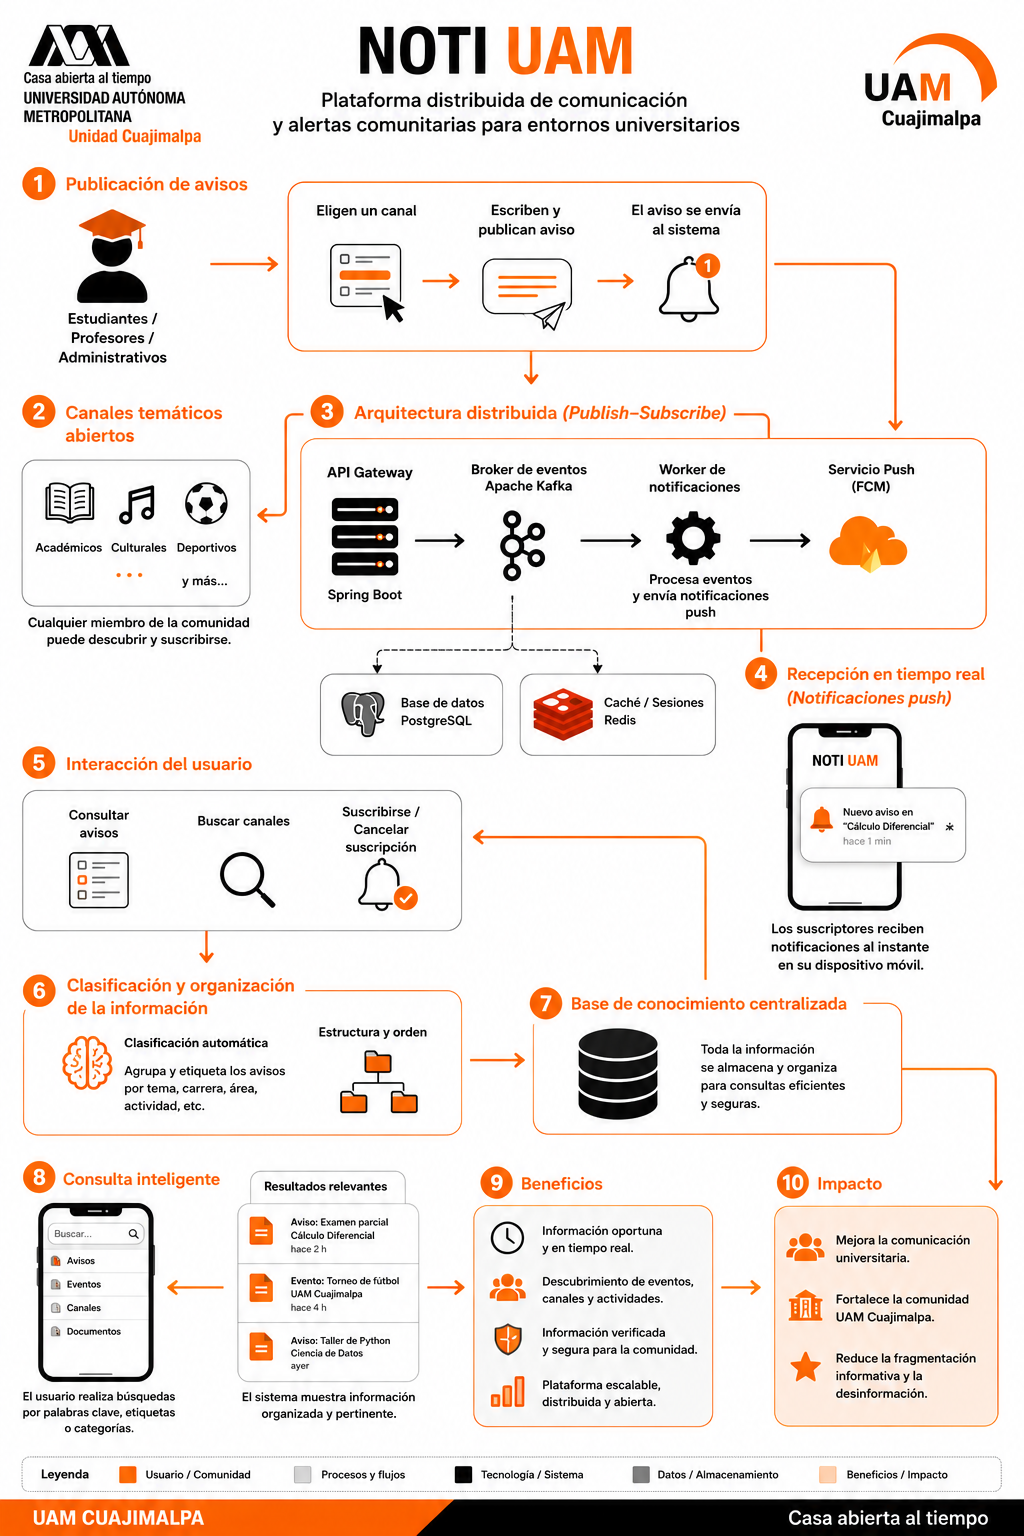
\includegraphics[width=.89\linewidth]{imagenes/arquitectura_componentes_cartel.png}
    \end{center}
    \end{block}
\end{minipage}

\end{minipage}

% ============================================================
% COL 2
% ============================================================

\begin{minipage}[t][0.3\textheight][t]{\textwidth}
\noindent\begin{tcolorbox}[colframe=white,colback=white,height=0.0cm,left=0pt,right=0pt,top=0pt,bottom=0pt,boxsep=0pt]
\end{tcolorbox}
 \vspace{-1.5cm}

\begin{minipage}[t]{0.48\textwidth}
\begin{block}{\Large 5. Estado del Arte}
Las características que diferencian a \emph{Noti Uam} de las soluciones existentes son:
\begin{table}[H]
\centering
\footnotesize
\setlength{\tabcolsep}{20pt}
\renewcommand{\arraystretch}{1.40}
\begin{tabular}{|l|c|c|c|c|}
\toprule
\textbf{Característica} & \textbf{WhatsApp} & \textbf{Telegram} & \textbf{UAM App} & \textbf{Noti Uam} \\
\midrule
Canales abiertos & No & Sí (públicos) & No & \textbf{Sí} \\
Notificaciones push & Sí & Sí & No & \textbf{Sí} \\
Arquitectura distribuida & No & No & No & \textbf{Sí (pub-sub)} \\
Autenticación institucional & No & Parcial (bots) & Sí & \textbf{Sí (JWT)} \\
Usabilidad validada & No & No & No & \textbf{Sí (pruebas SUS)} \\
Enfoque educativo & No & No & Sí (consulta) & \textbf{Sí (comunidad)} \\
\bottomrule
\end{tabular}
\end{table}
\end{block}

\begin{block}{\Large 6. Metodología}
Desarrollo incremental en 9 fases distribuidas en 3 trimestres (33 semanas):
\begin{itemize}[leftmargin=*]
    \item \textbf{PT I}: Análisis, diseño, entorno Docker, inicio del backend.
    \item \textbf{PT II}: Backend completo, base de datos, app móvil.
    \item \textbf{PT III}: Integración, pruebas de usabilidad (SUS) y rendimiento, documentación.
\end{itemize}
Se aplican encuestas, entrevistas y pruebas con estudiantes para validar la usabilidad y el rendimiento.
\end{block}

\end{minipage}\hspace{0.04\textwidth}%

\begin{minipage}[t]{0.46\textwidth}
\begin{block}{\Large 7. Resultados Esperados}
    \begin{itemize}[leftmargin=*]
        \item Una plataforma funcional que centralice la comunicación universitaria.
        \item Reducción de la fragmentación informativa y mejora en el descubrimiento de eventos.
        \item Notificaciones en tiempo real con latencia < 2 segundos.
        \item Aplicación móvil usable (puntuación SUS > 70) y accesible.
        \item Control total de la información por parte de la institución (privacidad y seguridad).
        \item Validación de la hipótesis: la arquitectura pub-sub mejora la difusión frente a herramientas genéricas.
    \end{itemize}
    \vspace{0.3cm}
    \textbf{Hipótesis:} \emph{“La implementación de Noti Uam reduce significativamente los tiempos de difusión y aumenta la participación estudiantil en comparación con WhatsApp y correo institucional.”}
\end{block}
\end{minipage}

\end{minipage}

\end{frame}
\end{document}